\documentclass[10pt]{article} % For LaTeX2e

% This template and styling file have been adapted from the ML Reproducibility Challenge 2020 and TMLR templates, to ease the submission.

% If you want to show the general instuctions, use the following command:
\usepackage[instructions]{atml}
% For the final version, use this one:
%\usepackage{atml}

% If you want to submit this work to tmlr, use the "tmlr" package rather than the "atml" one. Note: double-check the files needed in TMLR's submission instructions. 
% \usepackage{tmlr}
% If accepted, instead use the following line for the camera-ready submission:
%\usepackage[accepted]{tmlr}
% To de-anonymize and remove mentions to TMLR (for example for posting to preprint servers), instead use the following:
%\usepackage[preprint]{tmlr}

% Note that the following lines have been added to atml.sty:
% \usepackage[hidelinks]{hyperref}
% \newcommand*{\doi}[1]{\href{http://doi.org/#1}{doi: #1}}
% If atml.sty is not used, then these lines might need to be added to the respective styling files.
%%%%% NEW MATH DEFINITIONS %%%%%

\usepackage{amsmath,amsfonts,bm}

% Mark sections of captions for referring to divisions of figures
\newcommand{\figleft}{{\em (Left)}}
\newcommand{\figcenter}{{\em (Center)}}
\newcommand{\figright}{{\em (Right)}}
\newcommand{\figtop}{{\em (Top)}}
\newcommand{\figbottom}{{\em (Bottom)}}
\newcommand{\captiona}{{\em (a)}}
\newcommand{\captionb}{{\em (b)}}
\newcommand{\captionc}{{\em (c)}}
\newcommand{\captiond}{{\em (d)}}

% Highlight a newly defined term
\newcommand{\newterm}[1]{{\bf #1}}


% Figure reference, lower-case.
\def\figref#1{figure~\ref{#1}}
% Figure reference, capital. For start of sentence
\def\Figref#1{Figure~\ref{#1}}
\def\twofigref#1#2{figures \ref{#1} and \ref{#2}}
\def\quadfigref#1#2#3#4{figures \ref{#1}, \ref{#2}, \ref{#3} and \ref{#4}}
% Section reference, lower-case.
\def\secref#1{section~\ref{#1}}
% Section reference, capital.
\def\Secref#1{Section~\ref{#1}}
% Reference to two sections.
\def\twosecrefs#1#2{sections \ref{#1} and \ref{#2}}
% Reference to three sections.
\def\secrefs#1#2#3{sections \ref{#1}, \ref{#2} and \ref{#3}}
% Reference to an equation, lower-case.
\def\eqref#1{equation~\ref{#1}}
% Reference to an equation, upper case
\def\Eqref#1{Equation~\ref{#1}}
% A raw reference to an equation---avoid using if possible
\def\plaineqref#1{\ref{#1}}
% Reference to a chapter, lower-case.
\def\chapref#1{chapter~\ref{#1}}
% Reference to an equation, upper case.
\def\Chapref#1{Chapter~\ref{#1}}
% Reference to a range of chapters
\def\rangechapref#1#2{chapters\ref{#1}--\ref{#2}}
% Reference to an algorithm, lower-case.
\def\algref#1{algorithm~\ref{#1}}
% Reference to an algorithm, upper case.
\def\Algref#1{Algorithm~\ref{#1}}
\def\twoalgref#1#2{algorithms \ref{#1} and \ref{#2}}
\def\Twoalgref#1#2{Algorithms \ref{#1} and \ref{#2}}
% Reference to a part, lower case
\def\partref#1{part~\ref{#1}}
% Reference to a part, upper case
\def\Partref#1{Part~\ref{#1}}
\def\twopartref#1#2{parts \ref{#1} and \ref{#2}}

\def\ceil#1{\lceil #1 \rceil}
\def\floor#1{\lfloor #1 \rfloor}
\def\1{\bm{1}}
\newcommand{\train}{\mathcal{D}}
\newcommand{\valid}{\mathcal{D_{\mathrm{valid}}}}
\newcommand{\test}{\mathcal{D_{\mathrm{test}}}}

\def\eps{{\epsilon}}


% Random variables
\def\reta{{\textnormal{$\eta$}}}
\def\ra{{\textnormal{a}}}
\def\rb{{\textnormal{b}}}
\def\rc{{\textnormal{c}}}
\def\rd{{\textnormal{d}}}
\def\re{{\textnormal{e}}}
\def\rf{{\textnormal{f}}}
\def\rg{{\textnormal{g}}}
\def\rh{{\textnormal{h}}}
\def\ri{{\textnormal{i}}}
\def\rj{{\textnormal{j}}}
\def\rk{{\textnormal{k}}}
\def\rl{{\textnormal{l}}}
% rm is already a command, just don't name any random variables m
\def\rn{{\textnormal{n}}}
\def\ro{{\textnormal{o}}}
\def\rp{{\textnormal{p}}}
\def\rq{{\textnormal{q}}}
\def\rr{{\textnormal{r}}}
\def\rs{{\textnormal{s}}}
\def\rt{{\textnormal{t}}}
\def\ru{{\textnormal{u}}}
\def\rv{{\textnormal{v}}}
\def\rw{{\textnormal{w}}}
\def\rx{{\textnormal{x}}}
\def\ry{{\textnormal{y}}}
\def\rz{{\textnormal{z}}}

% Random vectors
\def\rvepsilon{{\mathbf{\epsilon}}}
\def\rvtheta{{\mathbf{\theta}}}
\def\rva{{\mathbf{a}}}
\def\rvb{{\mathbf{b}}}
\def\rvc{{\mathbf{c}}}
\def\rvd{{\mathbf{d}}}
\def\rve{{\mathbf{e}}}
\def\rvf{{\mathbf{f}}}
\def\rvg{{\mathbf{g}}}
\def\rvh{{\mathbf{h}}}
\def\rvu{{\mathbf{i}}}
\def\rvj{{\mathbf{j}}}
\def\rvk{{\mathbf{k}}}
\def\rvl{{\mathbf{l}}}
\def\rvm{{\mathbf{m}}}
\def\rvn{{\mathbf{n}}}
\def\rvo{{\mathbf{o}}}
\def\rvp{{\mathbf{p}}}
\def\rvq{{\mathbf{q}}}
\def\rvr{{\mathbf{r}}}
\def\rvs{{\mathbf{s}}}
\def\rvt{{\mathbf{t}}}
\def\rvu{{\mathbf{u}}}
\def\rvv{{\mathbf{v}}}
\def\rvw{{\mathbf{w}}}
\def\rvx{{\mathbf{x}}}
\def\rvy{{\mathbf{y}}}
\def\rvz{{\mathbf{z}}}

% Elements of random vectors
\def\erva{{\textnormal{a}}}
\def\ervb{{\textnormal{b}}}
\def\ervc{{\textnormal{c}}}
\def\ervd{{\textnormal{d}}}
\def\erve{{\textnormal{e}}}
\def\ervf{{\textnormal{f}}}
\def\ervg{{\textnormal{g}}}
\def\ervh{{\textnormal{h}}}
\def\ervi{{\textnormal{i}}}
\def\ervj{{\textnormal{j}}}
\def\ervk{{\textnormal{k}}}
\def\ervl{{\textnormal{l}}}
\def\ervm{{\textnormal{m}}}
\def\ervn{{\textnormal{n}}}
\def\ervo{{\textnormal{o}}}
\def\ervp{{\textnormal{p}}}
\def\ervq{{\textnormal{q}}}
\def\ervr{{\textnormal{r}}}
\def\ervs{{\textnormal{s}}}
\def\ervt{{\textnormal{t}}}
\def\ervu{{\textnormal{u}}}
\def\ervv{{\textnormal{v}}}
\def\ervw{{\textnormal{w}}}
\def\ervx{{\textnormal{x}}}
\def\ervy{{\textnormal{y}}}
\def\ervz{{\textnormal{z}}}

% Random matrices
\def\rmA{{\mathbf{A}}}
\def\rmB{{\mathbf{B}}}
\def\rmC{{\mathbf{C}}}
\def\rmD{{\mathbf{D}}}
\def\rmE{{\mathbf{E}}}
\def\rmF{{\mathbf{F}}}
\def\rmG{{\mathbf{G}}}
\def\rmH{{\mathbf{H}}}
\def\rmI{{\mathbf{I}}}
\def\rmJ{{\mathbf{J}}}
\def\rmK{{\mathbf{K}}}
\def\rmL{{\mathbf{L}}}
\def\rmM{{\mathbf{M}}}
\def\rmN{{\mathbf{N}}}
\def\rmO{{\mathbf{O}}}
\def\rmP{{\mathbf{P}}}
\def\rmQ{{\mathbf{Q}}}
\def\rmR{{\mathbf{R}}}
\def\rmS{{\mathbf{S}}}
\def\rmT{{\mathbf{T}}}
\def\rmU{{\mathbf{U}}}
\def\rmV{{\mathbf{V}}}
\def\rmW{{\mathbf{W}}}
\def\rmX{{\mathbf{X}}}
\def\rmY{{\mathbf{Y}}}
\def\rmZ{{\mathbf{Z}}}

% Elements of random matrices
\def\ermA{{\textnormal{A}}}
\def\ermB{{\textnormal{B}}}
\def\ermC{{\textnormal{C}}}
\def\ermD{{\textnormal{D}}}
\def\ermE{{\textnormal{E}}}
\def\ermF{{\textnormal{F}}}
\def\ermG{{\textnormal{G}}}
\def\ermH{{\textnormal{H}}}
\def\ermI{{\textnormal{I}}}
\def\ermJ{{\textnormal{J}}}
\def\ermK{{\textnormal{K}}}
\def\ermL{{\textnormal{L}}}
\def\ermM{{\textnormal{M}}}
\def\ermN{{\textnormal{N}}}
\def\ermO{{\textnormal{O}}}
\def\ermP{{\textnormal{P}}}
\def\ermQ{{\textnormal{Q}}}
\def\ermR{{\textnormal{R}}}
\def\ermS{{\textnormal{S}}}
\def\ermT{{\textnormal{T}}}
\def\ermU{{\textnormal{U}}}
\def\ermV{{\textnormal{V}}}
\def\ermW{{\textnormal{W}}}
\def\ermX{{\textnormal{X}}}
\def\ermY{{\textnormal{Y}}}
\def\ermZ{{\textnormal{Z}}}

% Vectors
\def\vzero{{\bm{0}}}
\def\vone{{\bm{1}}}
\def\vmu{{\bm{\mu}}}
\def\vtheta{{\bm{\theta}}}
\def\va{{\bm{a}}}
\def\vb{{\bm{b}}}
\def\vc{{\bm{c}}}
\def\vd{{\bm{d}}}
\def\ve{{\bm{e}}}
\def\vf{{\bm{f}}}
\def\vg{{\bm{g}}}
\def\vh{{\bm{h}}}
\def\vi{{\bm{i}}}
\def\vj{{\bm{j}}}
\def\vk{{\bm{k}}}
\def\vl{{\bm{l}}}
\def\vm{{\bm{m}}}
\def\vn{{\bm{n}}}
\def\vo{{\bm{o}}}
\def\vp{{\bm{p}}}
\def\vq{{\bm{q}}}
\def\vr{{\bm{r}}}
\def\vs{{\bm{s}}}
\def\vt{{\bm{t}}}
\def\vu{{\bm{u}}}
\def\vv{{\bm{v}}}
\def\vw{{\bm{w}}}
\def\vx{{\bm{x}}}
\def\vy{{\bm{y}}}
\def\vz{{\bm{z}}}

% Elements of vectors
\def\evalpha{{\alpha}}
\def\evbeta{{\beta}}
\def\evepsilon{{\epsilon}}
\def\evlambda{{\lambda}}
\def\evomega{{\omega}}
\def\evmu{{\mu}}
\def\evpsi{{\psi}}
\def\evsigma{{\sigma}}
\def\evtheta{{\theta}}
\def\eva{{a}}
\def\evb{{b}}
\def\evc{{c}}
\def\evd{{d}}
\def\eve{{e}}
\def\evf{{f}}
\def\evg{{g}}
\def\evh{{h}}
\def\evi{{i}}
\def\evj{{j}}
\def\evk{{k}}
\def\evl{{l}}
\def\evm{{m}}
\def\evn{{n}}
\def\evo{{o}}
\def\evp{{p}}
\def\evq{{q}}
\def\evr{{r}}
\def\evs{{s}}
\def\evt{{t}}
\def\evu{{u}}
\def\evv{{v}}
\def\evw{{w}}
\def\evx{{x}}
\def\evy{{y}}
\def\evz{{z}}

% Matrix
\def\mA{{\bm{A}}}
\def\mB{{\bm{B}}}
\def\mC{{\bm{C}}}
\def\mD{{\bm{D}}}
\def\mE{{\bm{E}}}
\def\mF{{\bm{F}}}
\def\mG{{\bm{G}}}
\def\mH{{\bm{H}}}
\def\mI{{\bm{I}}}
\def\mJ{{\bm{J}}}
\def\mK{{\bm{K}}}
\def\mL{{\bm{L}}}
\def\mM{{\bm{M}}}
\def\mN{{\bm{N}}}
\def\mO{{\bm{O}}}
\def\mP{{\bm{P}}}
\def\mQ{{\bm{Q}}}
\def\mR{{\bm{R}}}
\def\mS{{\bm{S}}}
\def\mT{{\bm{T}}}
\def\mU{{\bm{U}}}
\def\mV{{\bm{V}}}
\def\mW{{\bm{W}}}
\def\mX{{\bm{X}}}
\def\mY{{\bm{Y}}}
\def\mZ{{\bm{Z}}}
\def\mBeta{{\bm{\beta}}}
\def\mPhi{{\bm{\Phi}}}
\def\mLambda{{\bm{\Lambda}}}
\def\mSigma{{\bm{\Sigma}}}

% Tensor
\DeclareMathAlphabet{\mathsfit}{\encodingdefault}{\sfdefault}{m}{sl}
\SetMathAlphabet{\mathsfit}{bold}{\encodingdefault}{\sfdefault}{bx}{n}
\newcommand{\tens}[1]{\bm{\mathsfit{#1}}}
\def\tA{{\tens{A}}}
\def\tB{{\tens{B}}}
\def\tC{{\tens{C}}}
\def\tD{{\tens{D}}}
\def\tE{{\tens{E}}}
\def\tF{{\tens{F}}}
\def\tG{{\tens{G}}}
\def\tH{{\tens{H}}}
\def\tI{{\tens{I}}}
\def\tJ{{\tens{J}}}
\def\tK{{\tens{K}}}
\def\tL{{\tens{L}}}
\def\tM{{\tens{M}}}
\def\tN{{\tens{N}}}
\def\tO{{\tens{O}}}
\def\tP{{\tens{P}}}
\def\tQ{{\tens{Q}}}
\def\tR{{\tens{R}}}
\def\tS{{\tens{S}}}
\def\tT{{\tens{T}}}
\def\tU{{\tens{U}}}
\def\tV{{\tens{V}}}
\def\tW{{\tens{W}}}
\def\tX{{\tens{X}}}
\def\tY{{\tens{Y}}}
\def\tZ{{\tens{Z}}}


% Graph
\def\gA{{\mathcal{A}}}
\def\gB{{\mathcal{B}}}
\def\gC{{\mathcal{C}}}
\def\gD{{\mathcal{D}}}
\def\gE{{\mathcal{E}}}
\def\gF{{\mathcal{F}}}
\def\gG{{\mathcal{G}}}
\def\gH{{\mathcal{H}}}
\def\gI{{\mathcal{I}}}
\def\gJ{{\mathcal{J}}}
\def\gK{{\mathcal{K}}}
\def\gL{{\mathcal{L}}}
\def\gM{{\mathcal{M}}}
\def\gN{{\mathcal{N}}}
\def\gO{{\mathcal{O}}}
\def\gP{{\mathcal{P}}}
\def\gQ{{\mathcal{Q}}}
\def\gR{{\mathcal{R}}}
\def\gS{{\mathcal{S}}}
\def\gT{{\mathcal{T}}}
\def\gU{{\mathcal{U}}}
\def\gV{{\mathcal{V}}}
\def\gW{{\mathcal{W}}}
\def\gX{{\mathcal{X}}}
\def\gY{{\mathcal{Y}}}
\def\gZ{{\mathcal{Z}}}

% Sets
\def\sA{{\mathbb{A}}}
\def\sB{{\mathbb{B}}}
\def\sC{{\mathbb{C}}}
\def\sD{{\mathbb{D}}}
% Don't use a set called E, because this would be the same as our symbol
% for expectation.
\def\sF{{\mathbb{F}}}
\def\sG{{\mathbb{G}}}
\def\sH{{\mathbb{H}}}
\def\sI{{\mathbb{I}}}
\def\sJ{{\mathbb{J}}}
\def\sK{{\mathbb{K}}}
\def\sL{{\mathbb{L}}}
\def\sM{{\mathbb{M}}}
\def\sN{{\mathbb{N}}}
\def\sO{{\mathbb{O}}}
\def\sP{{\mathbb{P}}}
\def\sQ{{\mathbb{Q}}}
\def\sR{{\mathbb{R}}}
\def\sS{{\mathbb{S}}}
\def\sT{{\mathbb{T}}}
\def\sU{{\mathbb{U}}}
\def\sV{{\mathbb{V}}}
\def\sW{{\mathbb{W}}}
\def\sX{{\mathbb{X}}}
\def\sY{{\mathbb{Y}}}
\def\sZ{{\mathbb{Z}}}

% Entries of a matrix
\def\emLambda{{\Lambda}}
\def\emA{{A}}
\def\emB{{B}}
\def\emC{{C}}
\def\emD{{D}}
\def\emE{{E}}
\def\emF{{F}}
\def\emG{{G}}
\def\emH{{H}}
\def\emI{{I}}
\def\emJ{{J}}
\def\emK{{K}}
\def\emL{{L}}
\def\emM{{M}}
\def\emN{{N}}
\def\emO{{O}}
\def\emP{{P}}
\def\emQ{{Q}}
\def\emR{{R}}
\def\emS{{S}}
\def\emT{{T}}
\def\emU{{U}}
\def\emV{{V}}
\def\emW{{W}}
\def\emX{{X}}
\def\emY{{Y}}
\def\emZ{{Z}}
\def\emSigma{{\Sigma}}

% entries of a tensor
% Same font as tensor, without \bm wrapper
\newcommand{\etens}[1]{\mathsfit{#1}}
\def\etLambda{{\etens{\Lambda}}}
\def\etA{{\etens{A}}}
\def\etB{{\etens{B}}}
\def\etC{{\etens{C}}}
\def\etD{{\etens{D}}}
\def\etE{{\etens{E}}}
\def\etF{{\etens{F}}}
\def\etG{{\etens{G}}}
\def\etH{{\etens{H}}}
\def\etI{{\etens{I}}}
\def\etJ{{\etens{J}}}
\def\etK{{\etens{K}}}
\def\etL{{\etens{L}}}
\def\etM{{\etens{M}}}
\def\etN{{\etens{N}}}
\def\etO{{\etens{O}}}
\def\etP{{\etens{P}}}
\def\etQ{{\etens{Q}}}
\def\etR{{\etens{R}}}
\def\etS{{\etens{S}}}
\def\etT{{\etens{T}}}
\def\etU{{\etens{U}}}
\def\etV{{\etens{V}}}
\def\etW{{\etens{W}}}
\def\etX{{\etens{X}}}
\def\etY{{\etens{Y}}}
\def\etZ{{\etens{Z}}}

% The true underlying data generating distribution
\newcommand{\pdata}{p_{\rm{data}}}
% The empirical distribution defined by the training set
\newcommand{\ptrain}{\hat{p}_{\rm{data}}}
\newcommand{\Ptrain}{\hat{P}_{\rm{data}}}
% The model distribution
\newcommand{\pmodel}{p_{\rm{model}}}
\newcommand{\Pmodel}{P_{\rm{model}}}
\newcommand{\ptildemodel}{\tilde{p}_{\rm{model}}}
% Stochastic autoencoder distributions
\newcommand{\pencode}{p_{\rm{encoder}}}
\newcommand{\pdecode}{p_{\rm{decoder}}}
\newcommand{\precons}{p_{\rm{reconstruct}}}

\newcommand{\laplace}{\mathrm{Laplace}} % Laplace distribution

\newcommand{\E}{\mathbb{E}}
\newcommand{\Ls}{\mathcal{L}}
\newcommand{\R}{\mathbb{R}}
\newcommand{\emp}{\tilde{p}}
\newcommand{\lr}{\alpha}
\newcommand{\reg}{\lambda}
\newcommand{\rect}{\mathrm{rectifier}}
\newcommand{\softmax}{\mathrm{softmax}}
\newcommand{\sigmoid}{\sigma}
\newcommand{\softplus}{\zeta}
\newcommand{\KL}{D_{\mathrm{KL}}}
\newcommand{\Var}{\mathrm{Var}}
\newcommand{\standarderror}{\mathrm{SE}}
\newcommand{\Cov}{\mathrm{Cov}}
% Wolfram Mathworld says $L^2$ is for function spaces and $\ell^2$ is for vectors
% But then they seem to use $L^2$ for vectors throughout the site, and so does
% wikipedia.
\newcommand{\normlzero}{L^0}
\newcommand{\normlone}{L^1}
\newcommand{\normltwo}{L^2}
\newcommand{\normlp}{L^p}
\newcommand{\normmax}{L^\infty}

\newcommand{\parents}{Pa} % See usage in notation.tex. Chosen to match Daphne's book.

\DeclareMathOperator*{\argmax}{arg\,max}
\DeclareMathOperator*{\argmin}{arg\,min}

\DeclareMathOperator{\sign}{sign}
\DeclareMathOperator{\Tr}{Tr}
\let\ab\allowbreak


\usepackage{hyperref}
\usepackage{url}
\usepackage{tikz}
\usepackage{subcaption}
\usepackage[subpreambles=true]{standalone}
\usepackage{multirow}
\usepackage{multicol}

\title{ATML Report}

\author{%
  \name Jonatan Bella \email \href{mailto:jonatan.bella@usi.ch}{jonatan.bella@usi.ch}
  \AND
  \name Alessia Berarducci \email \href{mailto:alessia.berarducci@usi.ch}{alessia.berarducci@usi.ch}
  \AND
  \name Jonas Knupp \email \href{mailto:jonas.knupp@usi.ch}{jonas.knupp@usi.ch}
  \AND
  \name Tobias Erbacher \email \href{mailto:tobias.erbacher@usi.ch}{tobias.erbacher@usi.ch}
}

\def\groupid{Reinforcement Learning}
\def\projectid{RLE}


\begin{document}

\maketitle

\begin{abstract}
In this project we analyze the claims of \cite{rle-paper} in the paper \href{https://arxiv.org/abs/2407.13755}{\textsc{Random Latent Exploration for Deep Reinforcement Learning}}\footnote{Please note that there exists an older version of this paper by \cite{rle-paper-old} marked in the references with "(OLD VERSION)" which was provided by the course instructors. Only where there are significant differences we will refer to the new version.} which introduces a new technique to explore the state space and thus yield better overall agent scores. Moreover, we intend to reproduce the results obtained by the authors, expand on the findings and verify that the results are not cherry-picked. \textcolor{red}{<write the main findings of our project>} This report is prepared as part of the course project in \textit{Advanced Topics in Machine Learning} at \textit{Università della Svizzera italiana} in the autumn semester of 2024. \textcolor{red}{@ Update once we have all the findings}
\end{abstract}

%%%%

\section{Introduction}
\noindent The paper we investigate deals with the problem of motivating an agent in a high-dimensional state space to explore the environment more exhaustively during training and thereby find non-obvious trajectories that can lead to higher long-term rewards for both discrete and continuous action spaces. The paper compares the new \textit{Random Latent Exploration} (RLE) technique to standard \textit{Proximal Policy Optimization} (PPO, see \cite{ppo-paper}), \textit{NoisyNet} (see \cite{noisynet-paper}) and \textit{Random Network Distillation} (RND, see \cite{rnd-paper}).

\noindent Exploration is one of the major challenges of Reinforcement Learning (RL) and its techniques can generally be divided into two categories: Noise-based exploration and bonus-based exploration. There are advantages and disadvantages for both of them but we always have to keep in mind that always choosing the highest short-term (local) reward does not necessarily also yield the highest long-term (global) reward. E.g., picture the environment shown in figure \ref{fig:sample-env-1}. Here, the agent starting in the \textcolor{blue}{blue state} will always choose the small reward of $1$, i.e. going right, then move back to the initial state, then move right, and so on, dithering between these two states, instead of accepting to collect a reward of $0$ by going left in order to be able to collect the much higher reward of $100$ in the following step.

\noindent \cite{rle-paper} use RND to represent bonus-based exploration, NoisyNet to represent noise-based exploration and standard PPO as the baseline benchmark.

\begin{figure}[h!]
  \centering
  \begin{subfigure}[b]{0.45\textwidth}
    \centering
    \includegraphics[width=\textwidth]{tikz/sample-env-1.tex}
    \caption{Pure rewards.}
    \label{fig:sample-env-1}
  \end{subfigure}
  \hfill
  \begin{subfigure}[b]{0.45\textwidth}
    \centering
    \includegraphics[width=\textwidth]{tikz/sample-env-2.tex}
    \caption{Rewards with randomization (example).}
    \label{fig:sample-env-2}
  \end{subfigure}
  
  \caption{An exemplary environment consisting of four state where transitions can occur between neighboring states. The \textcolor{blue}{blue node} is the initial state and the numbers are the rewards.}
  \label{fig:sample-env}
\end{figure}

\newpage
\section{Scope of reproducibility}
\label{sec:claims}

\noindent The main quantifiable claims made by \cite{rle-paper} that we will be testing consist of the following:

\begin{enumerate}
    \item In the abstract, \cite{rle-paper} claim "[...] RLE exhibits higher overall scores across all of the tasks than other approaches, including action-noise and randomized value exploration", which they later specify for both "[...] discrete and continuous control tasks." They refer to the tasks being the \textsc{Atari}, \textsc{IssacGym} and \textsc{FourRoom} environments. The benchmark approaches are standard PPO, NoisyNet and RND.
    \item Moreover, "[...] introducting randomness to rewards influences the [... agent] to produce diverse behaviors" \citep{rle-paper} when this randomness is used to condition the policy and value networks, which manifests itself in an incentive to explore random (and thus in aggregate lager) parts of the state space.
    \item For the discrete-action discrete-states \textsc{FourRoom} environment absent of a goal reward, the authors claim that PPO's state visitation centers around the initial room (top right) concluding that action-noise methods cannot conduct deep exploration whereas RLE, NoisyNet and RND well reach across the four rooms and thus perform deep exploration.
    \item RLE performance improves over PPO irrespective of the distribution used to sample the 8-dim random latent vector.
\end{enumerate}

\noindent Our findings regarding these claims will be presented in \hyperlink{sec4}{section 4} \textcolor{red}{Check link before submission}. Please note that there are more claims made by the authors, however, due to time constraints we are not able to test all of them, the remaining ones are shown in \hyperlink{untested-claims}{appendix B} \textcolor{red}{check link before submission.}

\section{Methodology}
Random Latent Exploration --- The new idea that the authors \cite{rle-paper} present is to augment the reward function by adding a randomized term which incentivizes the agent to explore a larger portion of the state space. In particular, we will call this term $F(s, z)$ or intrinsic reward function, where $s \in \mathcal{S}$ is any state of the state space $\mathcal{S}$, and $\textbf{z} \in \mathbb{R}^{d}$ is a $d$-dimensional vector sampled from a given distribution $P_{\textbf{z}}$. The authors \cite{rle-paper} claim that RLE's efficiency is not significantly affected by the choice of $P_{\textbf{z}}$. If at time step $t \in \{0, 1, 2, ..., T\}$ the agent in state $s_{t}$ takes action $a_{t} \sim \pi(. | s_{t})$ from policy $\pi$, then it will obtain the task reward $r (s_{t}, a_{t})$. In RLE, we train a so-called latent-conditioned policy network $\pi(. | s, \textbf{z})$ and latent-conditioned value network $V^{\pi}(s, \textbf{z})$ to estimate and then maximize the expected sum of rewards from a given state, aware of the random term $z$:

\begin{equation}
    V^{\pi}(s, \textbf{z}) \approx \mathbb{E}_{\pi} \left[\sum_{t = 0}^{\infty} \gamma^{t} \left(r(s_{t}, a_{t}) + F(s_{t+1}, \textbf{z})\right) \right]
    \label{eq:value_func}
\end{equation}

\noindent In \eqref{eq:value_func}, $\gamma$ describes the discount factor and $F(s_{t+1}, \textbf{z}) =  \boldsymbol{\phi}(s) \cdot \textbf{z}$ where $\boldsymbol{\phi}(s): \mathcal{S} \rightarrow \mathbb{R}^{d}$ is a feature extraction network. The feature network is updated as a linear combination of the old feature network's weights and the weights of the value network\footnote{In the pseudocode algorithm in line 19 on page 25, in the mathematical formulation, the authors state that the feature network is updated as a linear combination of the old feature network's weights and the policy network's weights. We contacted the authors, and they confirmed that it should read $\phi \leftarrow \tau \cdot V^\phi + (1 - \tau ) \cdot \phi$ (i.e., the value network should be used, not the policy network). However, they state it would be interesting to explore which network should be used to update the feature network.}. Both $\boldsymbol{\phi}$ and $\textbf{z}$ are $d$-dimensional vectors. Note that although equation \ref{eq:value_func} is presented by \cite{rle-paper}, in the implementation they introduce an intrinsic and extrinsic reward coefficient. In the experiments they choose intrinsic reward coefficient $\ll$ extrinsic reward coefficient. Thus, they are not directly optimizing equation \ref{eq:value_func} in the experiments. Furthermore, on page 3 the authors state that $\vz$ "is resampled at the start of each trajectory". However, in the pseudocode on page 15 the authors note that $\vz$ is resampled at the end of each trajectory or after a certain number of steps has passed. Since the authors implemented the latter, more general, case we adopt the latter approach for our experiments. The authors split the critic's head into two: one head predicts the intrinsic value function, the other head predicts the extrinsic value function. Figure \ref{fig:rle-architecture} depicts how the action logits, intrinsic value, and extrinsic value for a given observation and $\vz$ is calculated. Note the residual connection from the first element-wise addition to the second element-wise addition. There is no mention of this residual connection in the paper. However, it is present in the provided code for the \textsc{Atari} environment. To continue the example from the introduction, in figure \ref{fig:sample-env-2} the agent would prioritize to go left as this promises the greater reward. It is not hard to imagine that for higher dimensional environments, every time we start a new trajectory and correspondingly sample a new $z$, the agent will explore a different region of the state space and thus we can discover non-obvious paths to maximize the rewards. For the detailed pseudocode of this algorithm, see \hyperlink{algo-rle}{Appendix A} \textcolor{red}{(check link before submmission)}.

\noindent A description of the other three algorithms can be found in \hyperlink{algo-ppo}{Appendix B} (PPO), \hyperlink{algo-noisynet}{Appendix C} (NoisyNet) and \hyperlink{algo-rnd}{Appendix D} (RND). Moreover, since the architecture of the neural networks we are using, e.g. for the feature extractor, value function approximation and policy, differ for each environment and every algorithm, we will explain them in \hyperlink{experimental-setup}{section 3.4} in detail. \textcolor{red}{(check all four links before submission)}

%\subsection{Datasets}

%\noindent Since we are dealing with a reinforcement learning task, we did not use any dataset to train our models but rather four different environments which will explain in \hyperlink{experimental-setup}{section 3.4} \textcolor{red}{(check link before submission)}.

\subsection{Hyperparameters}

\noindent In \textsc{Atari}, we mostly used the same values for the hyperparameters that the authors used. In table \ref{tab:atari-hyperparams} the hyperparameters we modified are summarized. Note that in the code, the z-sampling frequency is referred to as switch\_steps.

\begin{table}[h!]
  \centering
  \caption{Hyperparameters that differ from \cite{rle-paper} for the \textsc{Atari} experiments.}
  \begin{tabular}{{ll}} 
  \hline
  \textbf{Hyperparameter} & \textbf{Value} \\ \hline
  z-Sampling Frequency & 500\\ 
  Number of Runs per Game & 1 \\
  \end{tabular}
  \label{tab:atari-hyperparams}
\end{table}

\noindent \textcolor{red}{@Alessia: Are there undeclared hyperparameters in the code not listed in the paper?}

\noindent For the \textsc{FourRoom} experiments the hyperparameters stated in \cite{rle-paper} were used. However, \cite{rle-paper} did not provide values for all available hyperparameters. For the missing hyperparameters we used the values in table \ref{tab:gridworld-missing-hyperparameters}, that seemed reasonable to us although we did not spend a lot of time finetuning them.

\begin{table}[h!]
  \centering
  \caption{Hyperparameters not stated by \cite{rle-paper} for the \textsc{FourRoom} experiments.}
  \begin{tabular}{{ll}} 
  \hline
  \textbf{Hyperparameter} & \textbf{Value} \\ \hline
  Extrinsic Reward Coefficient & 1\\ 
  Observation Normalization Iterations & 1 \\
  Discount Rate & 0.99 \\ 
  Intrinsic Discount Rate & 0.99 \\ 
  Feature Network Update Rate $\tau$ & 0.005 \\ 
  Learning Rate & 0.001 \\ 
  \end{tabular}
  \label{tab:gridworld-missing-hyperparameters}
\end{table}

\noindent \textcolor{red}{@Jonathan: We need your input here for IsaacLab: Are all of the hyperparameters you used the ones from the RLE paper, or did you change/add/remove some of them, if yes which ones, what are their values and did you finetune them (how, what was the tuning range, how many different values did you try out)?}

\hypertarget{experimental-setup}{\subsection{Experimental setup and code}}

\noindent The code for our implementations can be found in GitHub\footnote{\href{https://github.com/jonupp/adv_topics_ml_repl_chal}{https://github.com/jonupp/adv\_topics\_ml\_repl\_chal} \textcolor{red}{Change github}}. There are three types of environments in use on which we run our RL algorithms which are depicted in figure \ref{fig:environmnents}. 


\noindent The authors of the paper at hand published code in a GitHub repository\footnote{\href{https://github.com/Improbable-AI/random-latent-exploration}{https://github.com/Improbable-AI/random-latent-exploration}}. This repository contains code for the \textsc{Atari} and \textsc{IsaacGym}\footnote{Please note that the \textsc{IsaacGym} environment is deprecated and we are using \textsc{IsaacLab} instead, however we will refer to it as \textsc{IsaacGym} for reasons of continuity.} environments with the 4 algorithms (RLE, PPO, RND, NoisyNet). 

\subsubsection{Atari}

\noindent The authors of the paper under investigation chose the \textsc{Atari} environment, introduced by \cite{atari-introduction}, to represent a discrete action-space deep-RL benchmark. This environment comprises $57$ different games, among which we performed experiments on two games, namely \textsc{Alien} and \textsc{StarGunner}. To understand the code given by the authors, we made use mainly of the official environment documentation as well as other papers that we found along the way. Here, the agent perceives the $4$ most recent $84\times84$ grayscale frames, one frame of which can be found in figure \ref{fig:sample-env-atari}. During training, every trajectory (episode) always commences from the same initial state and can be terminated in one of the two ways: A game event occurs, or the maximum episode length is reached. The former refers to e.g. the loss of a "life" or a task being completed. As the authors provided the code for this environment, we did not modify it significantly. The main claims that we tested here were the superior performance of RLE and deeper exploration.\\

\noindent The game score $S_{G}$ that we use to compare the different algorithms we run in this environment are normalized in the manner introduced by \cite{agent57} by taking into account the score an average human achieves $S_{H}$ as well as the score an agent achieves by always choosing a random action $S_{R}$, which gives us the human normalized score $S_{N} = \frac{S_{G} - S_{R}}{S_{H} - S_{R}}$. According to \cite{agent57}, in the case of \textsc{Alien}, we have $S_{H} = 7127.7$ and $S_{R} = 227.8$ while for \textsc{StarGunner} we have $S_{H} = 10250$ and $S_{R} = 664$. With the normalization we can get a better comparison of how much the agent behaves like a random agent ($S_{N} = 0$) or like a human player ($S_{N} = 1$), or even better $S_{N} > 1$. Moreover, the normalization allows for comparisons between games, adjusted for the general difficulty of a game.\\

\noindent Each game was run with all four algorithms (RLE, PPO, NoisyNet, RND) and the most important comparative measure to evaluate the agent's performance is the game score, which was computed from the cumulative extrinsic rewards (obtained from $\text{infos["r"]}$ of the environment) over the episodes, treated as undiscounted sums to ensure a uniform weight across time steps for the purpose of investigating the algorithm's exploratory abilities. To this end, we also record the time evolution of the Shannon entropy of each algorithm, where a higher entropy indicates that the agent's selection of actions out of all available actions is broader and less concentrated, hinting at more thorough exploration capabilities.\\

\textcolor{red}{@Who it may concern: trajectory length longer in RLE, compensating lower rewards?}

\subsubsection{FourRoom}
Figure \ref{fig:sample-env-fourroom} shows the \textsc{FourRoom} environment where we have $50\times50 + 4$ states\footnote{In \cite{rle-paper}, the authors claim that there are $50\times 50$ states. We contacted the authors, and they confirmed that it should read $50\times 50 + 4$ states.} which are divided into four rooms of size $25\times25$ and $4$ holes in the walls located at positions $10$ horizontally and $5$ vertically, starting the count at $1$ from the inner corners. Exploring the state space, beginning from the initial state marked in \textcolor{red}{red}, becomes a deep exploration task due to the holes being only $1$ "pixel" wide. However, if we want to incentivize the agent to find a reward, then we can put it at the goal position marked in \textcolor{green}{green}. The \textsc{FourRoom} environment was implemented such that we can pass a flag to the environment's constructor to choose whether the environment is reward-free or has the goal in the bottom-left corner. At every step, the agent can move one step vertically or horizontally, but if it would run into a wall it chooses to remain in place. \cite{rle-paper} refer to \cite{grid-world-paper} when introducing the \textsc{FourRoom} environment. \cite{grid-world-paper} use action stochasticity. We asked Mr. Mahankali whether they also used action stochasticity, and they stated that they did not use action stochasticity in their experiments. 

The authors did not provide any code for the \textsc{FourRoom} environment, so this environment was implemented by us using the gymnasium library introduced by \cite{gymnasium-paper} together with our adaptation of the code for PPO, NoisyNet and RLE algorithms from the \textsc{Atari} environment, while we adapted the RLE code from the \textsc{IsaacGym} environment. A wrapper to record the state visitation counts per environment was also implemented. Before we adapted RLE from the existing implementation for the \textsc{Atari} environment, we implemented it based on the description in \cite{rle-paper}. However, the paper lacked a lot of details present in the \textsc{Atari} code (e.g., split critic's head, residual connection) so that we decided to proceed with the adapted code to have consistent results over the different environments. 

First we investigate how RLE performs in a reward-free setting in comparison to PPO, NoisyNet, and RND. \cite{rle-paper} claims that RLE shows good explorative behavior based on a single heatmap of state visitation counts. To assess whether this result is expected or exceptional we trained each algorithm 20 times. Since it is not reasonable to compare 20 state visitation count heatmaps we used the Shannon entropy, introduced by \cite{shannon-entropy-paper}, of the state visitation counts as a proxy for how well an agent explored the environment. With increasing entropy the distribution of the state visitation counts becomes more uniform. Thus, the higher the entropy the better the explorative behavior. 

We also ran RLE, PPO, NoisyNet, and RND in the \textsc{FourRoom} environment with a goal to see how RLE compares to the other algorithms in an environment with a reward. Similar to the reward-free setting, we run each algorithm 20 times on different seeds. However, instead of assessing the performance of the algorithms using the Shannon entropy, we use the average game score. The game score is the average undiscounted return over the last 128 episodes. The average game score for a certain algorithm is the average of the game scores in the different runs for this algorithm.

Furthermore, it was explored if the intrinsic reward function really guides the generation of diverse trajectories in a reward-free environment. To assess this, the intrinsic value function for four latent vectors $z$ and four trajectories generated using the same latent vector $z$ were saved at the end of each experiment. 

We also tested to what degree RLE is indifferent to the distribution of the latent vector. To test this, we ran RLE with different latent vector distributions. The following distributions were considered: standard normal distribution, standard uniform distribution, Von-Mises distribution with $\mu=0$ and $\kappa=0.3$, and the exponential distribution with $\lambda=0.3$. We ran 20 experiments for each latent vector distribution and recorded the state visitation entropy. The same hyperparameters were used as before. Note that all latent vectors were normalized using the L2-norm, so that all latent vectors are on a unit sphere around the origin. This ensures that all intrinsic rewards are in the interval [-1,1]. \cite{rle-paper} performed a similar ablation study for the \textsc{Atari} environment. However, they did not normalize the latent vectors for all distributions. They only applied normalization for the normal distribution which they then denoted as "Sphere". They then compare the "Sphere" to the unnormalized uniform distribution and the unnormalized normal distribution. We normalized all distributions because the extrinsic reward coefficient and the intrinsic reward coefficient hyperparameters already control the weighting between the intrinsic and extrinsic rewards, so we wanted the intrinsic rewards to be in the interval [-1,1].


\subsubsection{IsaacGym}
\textcolor{red}{@Jonathan explain environment and experiments (NOT RESULT)}

\begin{figure}
  \centering
  \begin{subfigure}[b]{0.32\textwidth}
    \centering
    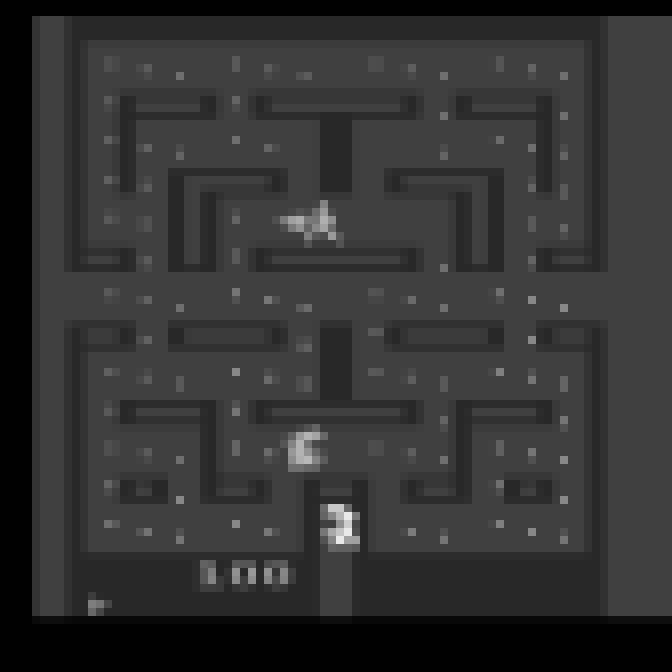
\includegraphics[width=\textwidth]{figures/atari.png}
    \caption{The \textsc{Alien-v5} environment is an example of the \textsc{Atari} games consisting of a maze filled with 'eggs' to destroy while being hunted by aliens. A flamethrower or occasional power-up may be used to scare the aliens.}
    \label{fig:sample-env-atari}
  \end{subfigure}
  \hfill
  \begin{subfigure}[b]{0.32\textwidth}
    \centering
    \includegraphics[width=\textwidth]{tikz/fourroom-env.tex}
    \caption{The \textsc{FourRoom} environment is a grid world, limited by walls, with the initial state is on the \textcolor{red}{top right} and the goal state where the agent receives a reward (optional) is on the \textcolor{green}{bottom left}.}
    \label{fig:sample-env-fourroom}
  \end{subfigure}
  \hfill
  \begin{subfigure}[b]{0.32\textwidth}
    \centering
    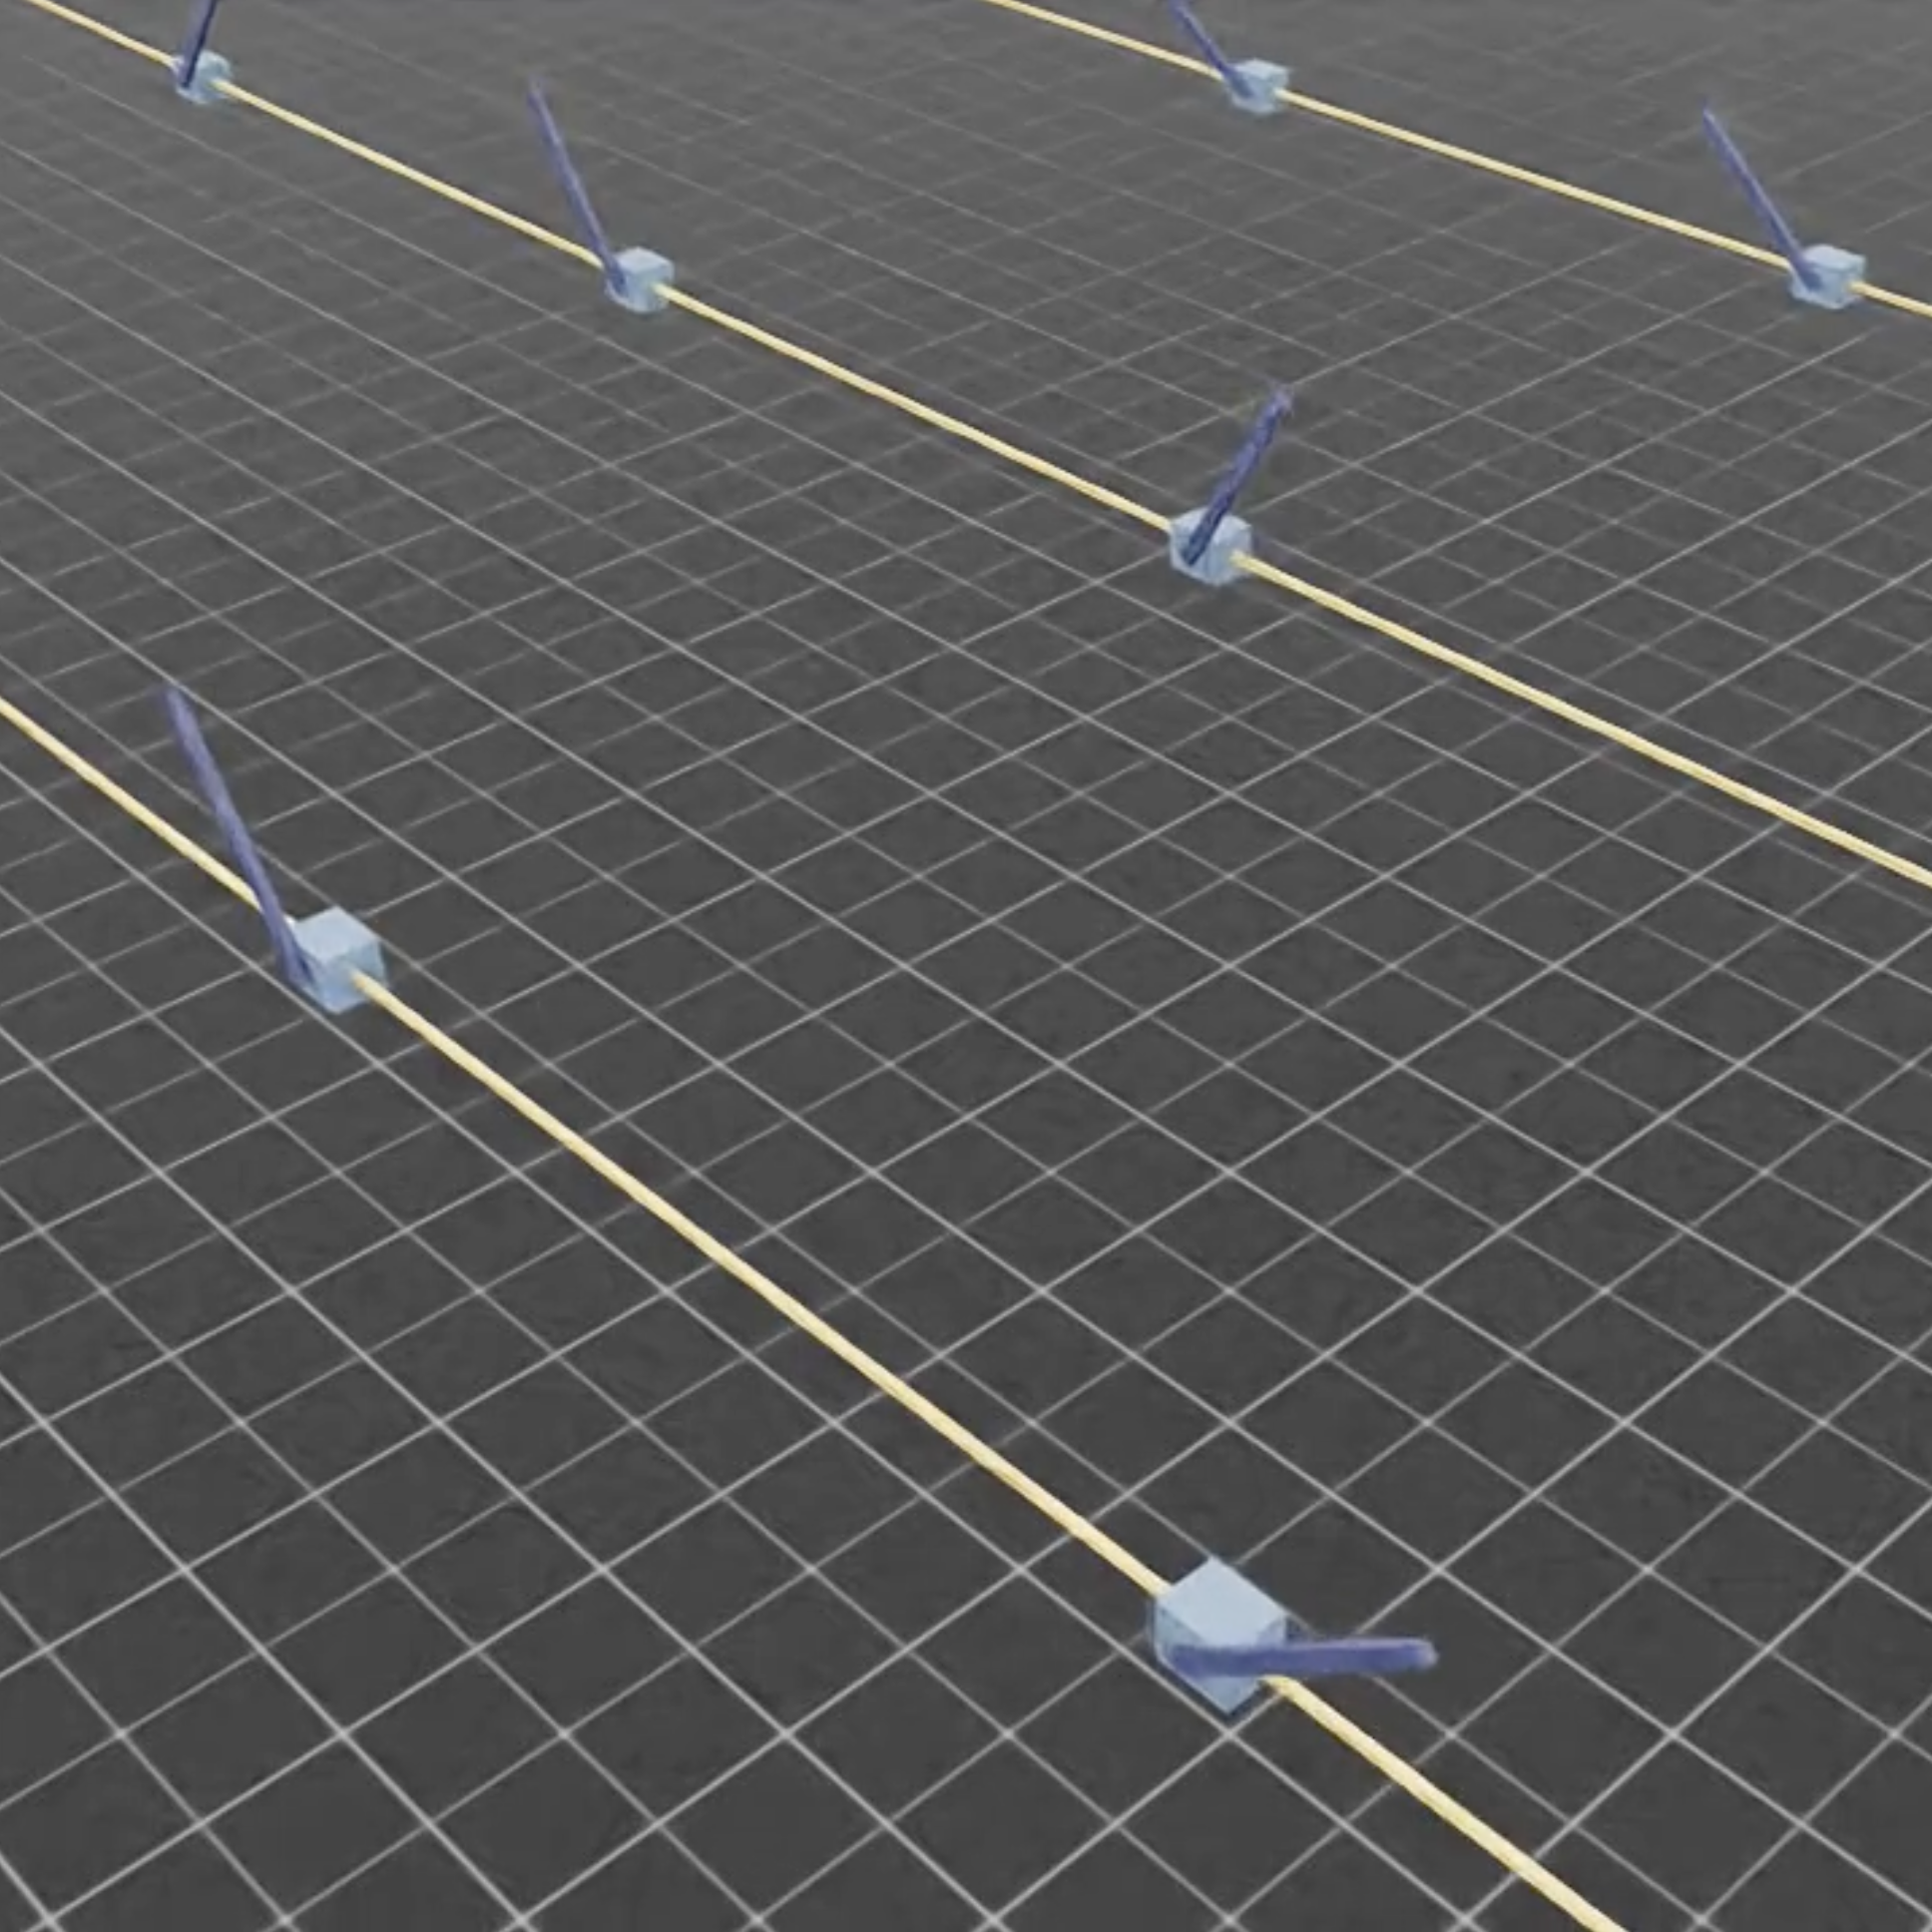
\includegraphics[width=\textwidth]{figures/isaac.png}
    \caption{The \textsc{CartPole} environment is an example of the \textsc{IsaacGym} environment.\\\textcolor{red}{What does the agent actually perceive?}\\}
    \label{fig:sample-env-isaac}
  \end{subfigure}
  \caption{Examples of the environments in use.}
  \label{fig:environmnents}
\end{figure}


\subsubsection{Queue-Based Von Mises-Fisher}
\cite{rle-paper} suggest it might be worthwhile to explore using a latent vector distribution that changes during the training. Our hypothesis is that at the start of the training the latent vector distribution $P_{\textbf{z}}$ should provide diverse $\textbf{z}$ since the agent should explore the environment. However, with increasing training progress, the agent should put less emphasis on exploration. We use the Von Mises-Fisher distribution with the parameters $\vmu$, the mean direction, and $\kappa$, the concentration to model $P_{\textbf{z}}$. The idea is to slowly change $\vmu$ during the training, so that it points to a point in the space such that $P_{\textbf{z}}$ samples $\mathbf{z}$ values that yield high returns. Furthermore, $\kappa$ should be slowly increased during the training to increase the probability to sample $\mathbf{z}$ close to $\vmu$. Since PyTorch does not provide an implementation to sample from this distribution, we used the implementation described by \cite{von-mises-fisher-paper} that is based on rejection sampling. We maintain a queue of $\textbf{z}$ values with good episodic return and a queue with the respective returns. After every finished episode, the queues are updated if necessary. We then update $\vmu$ as a linear combination of the $\textbf{z}$ values in the success memory. The weighting is done using the returns in the returns memory. $\kappa$ should be large if the model has converged to a $\vmu$ that reliably gives $\textbf{z}$ values with high returns. Thus, $\kappa$ is updated by linearly interpolation between 0 and 30. The weight is the average pairwise cosine similarity between the $\textbf{z}$ values in the success memory.


\subsubsection{Neural Adaptive Von Mises-Fisher}
\textcolor{red}{@Jonathan}


\hypertarget{computational-requirements}{\subsection{Computational requirements}}

\noindent All \textsc{FourRoom} experiments were performed on an Apple M2 Pro with 16 GB RAM. Every experiment was conducted in the reward-free environment and in the environment with a goal. Every algorithm and every RLE variant with different latent vector distribution was run 20 times with different seeds in each of the two environments. This resulted in a total of 280 runs. It took ca. 1 minute to do a single PPO run, ca. 1 minute and 20 seconds to do a single NoisyNet run, ca. 2 minutes to do a single RLE run, and ca. 2 minutes and 20 seconds to do a single RND run. The experiments for the different algorithms took at total time of ca. 4.4 hours. In addition, we trained RLE with three different latent vector distributions (apart from the standard normal distribution). These experiments took ca. 4 hours. Thus, the total computing time for all \textsc{FourRoom} experiments amounts to ca. 8.4 hours.

\noindent All experiments in the \textsc{Atari} environment were run in \href{https://colab.research.google.com/}{Google Colab}. Here we experimented with the available CPU, T4 GPU and TPU v2-8 and used Weights \& Biases (W\&B) for a real-time visualization of the game scores and other measures. In the end we chose the GPU for all runs. We linked a \href{https://drive.google.com}{Google Drive} to Colab in order to save model checkpoints. Overall the W\&B workspace now contains 56 runs with a total compute time of ca. $241.2$ hours, of which we are using 8 runs for the results of this project. Of that amount, ca. $76.7$ compute hours were spent on \textsc{StarGunner}, the remaining ca. $164.5$ compute hours were spent on \textsc{Alien}.

\noindent \textcolor{red}{@Jonatan: We need your input here for Isaac: Did you run all of the experiments on your mac/other laptop or did you use colab as well (which CPU or GPU was used (name))? What are the average training times e.g. per episode or global step? How many runs did you do overall (i.e. how many compute hours did you spend on this project) for each of the algorithms?}

\noindent We would like to note, however, that \cite{rle-paper} had the HPC resources of the MIT Supercloud and the Lincoln Laboratory Supercomputing Center available. Within the framework of this course, we did not have the equivalent computing power to replicate all experiments in their original form and had to restrain ourselves to a mere few of them.

\hypertarget{sec4}{\section{Results}}
\textcolor{red}{all figures in appendix as first item}

\noindent \texttt{Start with a high-level overview of your results. Do your results support the main claims of the original paper? Keep this section as factual and precise as possible, and reserve your judgment and discussion points for the next "Discussion" section.}


\subsection{Results reproducing original paper}
\texttt{For each experiment, say (1) which claim in Section~\ref{sec:claims} it supports, and (2) if it successfully reproduced the associated experiment in the original paper.}
\texttt{For example, an experiment training and evaluating a model on a dataset may support a claim that that model outperforms some baseline.}
\texttt{Logically group related results into subsections.}

\subsubsection{FourRoom}
The results from the experiment where every algorithm is run 20 times in the reward-free environment can be seen in figure \ref{fig:gridworld-entropy-algorithms}. RLE shows the best performance, followed by RND, NoisyNet and PPO. Furthermore, RLE has the narrowest confidence interval. Although \cite{rle-paper} did not perform an equivalent experiment, they concluded from the state visitation heatmap that RLE shows the best explorative behavior in this setting. This aligns with the result from our experiment. 

Figure \ref{fig:gridworld-score-algorithms} shows the result of the experiment where every algorithm is run 20 times in the environment with a goal. \cite{rle-paper} train five seeds in the environment with a goal for each algorithm, and find that the average score for RLE and NoisyNet is 0.6, while the average score for RND and PPO is 0. In our experiment RLE achieved the highest game score by a large margin while NoisyNet and RND performed similarly poorly with an average game score of $<0.2$ at the end of the training. PPO achieved an average game score of 0 at the end of the training. Thus, the result that RLE is among the best performing algorithms in this setting is confirmed by our experiment.

Figure \ref{fig:gridworld-entropy-distributions} depicts the result of the experiment where RLE variants with different latent vector distributions are compared in the reward-free environment by running each RLE variant 20 times. The RLE variants where the latent vector distribution follows the standard normal or Von Mises distribution perform similarly well and clearly outperform the RLE variants with standard uniform and exponential distribution. Moreover, the RLE variants with standard uniform and exponential distribution show similar performance to RND. These results indicate that the choice of the latent vector distribution is of some importance. Moreover, there are two pairs of distributions that show similar behavior although the distributions in the pair are not that similar. For instance, we chose parameters for the Von Mises distribution to make its peak small, so that it is quite different from a standard normal distribution and shows some similarity to a uniform distribution. 

In figure \ref{fig:gridworld-score-distributions} the results of the experiment where RLE variants with different latent vector distributions are compared in the environment with rewards. Again, each RLE variant was run 20 times. The RLE variant with the Von Mises distribution performs best, followed by the standard normal variant, the exponential variant, and lastly the standard uniform variant. The difference in average game score between the RLE variants is large: the worst variant achieves an average game score slighlty above 0.2 while the best RLE variant achieves an average game score of appr. 0.8. The ranking of the RLE variants is the same as in the experiment described before. Again, the results indicate that the choice of the latent vector distribution impacts the performance of RLE.

We generated state visitation heatmaps for each algorithm and RLE variant for both the reward-free environment and the environment with a goal. From the 20 runs for each algorithm and RLE variant we chose the run with the highest entropy in the case of the reward-free environment and the run with the highest game score in the case of the environment with a goal. In figure \ref{fig:gridworld-heatmap-nogoal-algorithms} the state visitation heatmaps for the different algorithms in the reward-free environment are displayed. RLE and NoisyNet explore all four rooms while PPO and RND have a significant number of unexplored states. Figure \ref{fig:gridworld-heatmap-nogoal-algorithms} shows the state visitation heatmaps for the different algorithms in the environment with a goal. RLE, NoisyNet, and RND are frequently visiting states on a appr. shortest path from the start to the goal while PPO has only explored a single room. Next, the state visitation for the RLE variants are considered. In figure \ref{fig:gridworld-heatmap-nogoal-distributions} we see that the standard normal, Von Mises, and exponential RLE variants explore all the four rooms well. Only the standard uniform RLE variant does not explore all states. In figure \ref{fig:gridworld-heatmap-goal-distributions} we see that all RLE variants often visit states on one of the appr. shortest path between start and goal. However, the standard normal and Von Mises variants explore almost the entire state space while the standard uniform and exponential RLE variants have large unexplored chunks.

Lastly, figure \ref{fig:gridworld-value-function-trajectories} shows that the intrinsic reward function guides the generation of diverse trajectories. The trajectories converge to areas where the intrinsic reward is large. 

All the 95\% confidence intervals are calculated using the bootstrapping method. 

\subsubsection{Atari}

\noindent After running each game for a total of $40$ million time steps, we have obtained the results shown in table \ref{tab:atari-results}.

\begin{table}[h!]
  \centering
  \caption{Results of the \textsc{Atari} experiments.}
  \begin{subtable}[h]{0.48\textwidth}
      \centering
      \begin{tabular}{{llll}} 
        \hline
        \textbf{Algorithm} & & Game Score & Human-Norm.\\
        \hline
        RLE & & $1626$ & $0.203$\\ 
        PPO & & $1384$ & $0.168$\\
        NoisyNet & & $648$ & $0.061$\\
        RND & & $1048$ & $0.119$\\
    \end{tabular}
    \caption{The \textsc{Alien} game.}
    \label{tab:alien-score}
  \end{subtable}
  \hfill
  \begin{subtable}[h]{0.48\textwidth}
      \centering
      \begin{tabular}{{llll}} 
        \hline
        \textbf{Algorithm} & & Game Score & Human-Norm.\\
        \hline
        RLE & & $42481$ & $4.362$\\ 
        PPO & & $54564$ & $5.623$\\
        NoisyNet & & $27530$ & $2.803$\\
        RND & & $21565$ & $2.180$\\
    \end{tabular}
    \caption{The \textsc{StarGunner} game.}
    \label{tab:stargunner-score}
  \end{subtable}
  \label{tab:atari-results}
\end{table}

\noindent For the \textsc{Atari} game, as can be seen in table \ref{tab:alien-score}, the algorithm perform in a similar manner to the authors' result. Only NoisyNet performs much worse in our run, obtaining a score of $648$, while the authors report a score of approximately $1113$. However, regarding claim $(1)$ we can confirm that RLE obtains the highest score of them all, which is evident from the plot of human-normalized scores in figure \ref{fig:alien-score}. Additionally, we can compare the depth of exploration done by these algorithms in figure \ref{fig:alien-entropy} by looking at the entropy distribution. Here, it is evident that RLE explores the largest part of the state space in comparison to the other algorithms. Using entropy as a measure of diverse behavior, we can moreover confirm as well claim $(2)$ for this game.\\

\noindent In the case of the \textsc{StarGunner} game, as becomes apparent in table \ref{tab:stargunner-score}, the RLE algorithm does not yield the best game score but PPO does. This result differs strongly from the findings of the authors. In more detail, we find that RLE obtains a game score of around $42481$ while the authors report $64011$, and in addition their implementation of NoisyNet performs much better at $42645$ while our agent only got $27530$ in the end. Thus, in this case we have to object claim $(1)$, which is shown in more detail in figure \ref{fig:stargunner-score}. On the contrary, we can confirm claim $(2)$ again as shown in figure \ref{fig:stargunner-entropy} since RLE does exhibit the most diverse behavior out of all four algorithms. Perhaps this hints at instabilities in the algorithmic behavior of the agent which are depending on e.g. the seed with which the run was initialized.

\subsubsection{IsaacGym}
\textcolor{red}{@Jonathan}


\subsection{Results beyond original paper}
\texttt{Often papers don't include enough information to fully specify their experiments, so some additional experimentation may be necessary. For example, it might be the case that batch size was not specified, and so different batch sizes need to be evaluated to reproduce the original results. Include the results of any additional experiments here. Note: this won't be necessary for all reproductions.}

\subsubsection{Atari}

\noindent One interesting observation that we made during our experiments is the fact that in \textsc{Alien}, the agent seems to obtain lower rewards on average with RLE, see figure \ref{fig:alien-rewards}, but still has the highest game score overall. We conjecture that this means the agent with RLE behaves more cautiously trying to stay alive for longer and collect lower/safer rewards but over a longer time horizon meaning the overall accumulated reward (game score) still turns out to be superior compared to the other algorithms. This would be confirmed by RLE having the largest trajectory (episode) length, see figure \ref{fig:alien-trajectorylength}. However, this is probably not the entire explanation, since in \textsc{StarGunner}, see figure \ref{fig:stargunner-rewards} and \ref{fig:stargunner-trajectorylength}, RLE also gets very low reward on average but here this cannot be compensated by having the largest trajectory length. Moreover, given that we also normalized the game scores, the result suggests that the agent is better at playing \textsc{StarGunner} and worse at playing \textsc{Alien} compared to an average human.

\subsubsection{Adaptive Von Mises-Fisher}
\textcolor{red}{@Jonathan}


\section{Discussion}
\textcolor{red}{Discuss claims}


\texttt{Give your judgment on if your experimental results support the claims of the paper. Discuss the strengths and weaknesses of your approach - perhaps you didn't have time to run all the experiments, or perhaps you did additional experiments that further strengthened the claims in the paper.}

\subsection{What was easy}
\textcolor{red}{@Tobias}

- Atari code was ready to run. 
- The concept of the paper is not hard to understand (also mathematically)

\texttt{Give your judgment of what was easy to reproduce. Perhaps the author's code is clearly written and easy to run, so it was easy to verify the majority of original claims. Or, the explanation in the paper was really easy to follow and put into code.}

\texttt{Be careful not to give sweeping generalizations. Something that is easy for you might be difficult for others. Put what was easy in context and explain why it was easy (e.g. code had extensive API documentation and a lot of examples that matched experiments in papers).}

\subsection{What was difficult}
A major challenge we faced was evaluating RLE across three distinct environments, each presenting unique difficulties. For the FourRoom environment, no implementation was available, requiring us to develop one from scratch. We aimed to replicate the approach used by \cite{rle-paper} as closely as possible to ensure comparability. The Atari environment, on the other hand, could be used without modification, but training agents demanded substantial computational resources. \textcolor{red}{@Jonathan add something about Isaac here.} Furthermore, in the paper, an important implementation detail, the split critic's head, is omitted. The paper itself also contains some contradicting information (\textsc{Atari} feature network size, condition to resample z) and minor errors (\textsc{FourRoom} environment description and typo in pseudocode regarding feature network update). Lastly, as RLE builds upon PPO with optimizations such as generalized advantage estimation, we had to dedicate considerable time to thoroughly understand the underlying PPO framework. 


\subsection{Communication with original authors}

\noindent During our replication study, a number of questions, mainly regarding parameters and model/environment architecture, came up which we were unable to answer by ourselves, so we sent an email to Mr. Mahankali. and got a response a few days later. Our questions and Mr. Mahankali's answers will be provided upon request. 

\section{Conclusion}
\texttt{Try to summarize the achievements of your project and its limits, suggesting (when appropriate) possible extensions and future works.}

\section*{Member contributions}

\noindent We divided the workload among the group members as follows:

\begin{itemize}
  \item Jonatan Bella: \textsc{IsaacLab} implementation, \textcolor{red}{please let me know what you want to add}
  \item Alessia Berarducci: \textsc{Atari} implementation, \textcolor{red}{please let me know what you want to add}
  \item Jonas Knupp: Implementation of the \textsc{FourRoom} environment, adaption of PPO, NoisyNet, RLE, and RND to the \textsc{FourRoom} environment, conducting the experiments with the \textsc{FourRoom} environment
  \item Tobias Erbacher: Report writing, project management, numpy-visualization.
\end{itemize}

\noindent However, we met regularly and assisted each other in their tasks so the split is not completely clear-cut.

%%%%

\bibliography{main}
\bibliographystyle{tmlr}

\appendix
\section{Appendix}
You may include other additional sections here. Here we provide suggestions and instructions for the layout and styling of the report.

\section{Citations, figures, and tables}

\paragraph{Citations}

When the authors or the publication are
included in the sentence, the citation should not be in parenthesis, using \verb|\citet{}| (as
in ``See \citet{Hinton06} for more information.''). Otherwise, the citation
should be in parenthesis using \verb|\citep{}| (as in ``Deep learning shows promise to make progress
towards AI~\citep{Bengio+chapter2007}.'').

\paragraph{Figures}

All artwork must be neat, clean, and legible. The figure number and caption always appear after the figure. Place one line space before the figure caption, and one line space after the figure. The figure caption is lowercase (except for the first word and proper nouns). Make sure the figure caption does not get separated from the figure. Leave sufficient space to avoid splitting the figure and figure caption.

\begin{figure}[ht]
\begin{center}
\fbox{\rule[-.5cm]{0cm}{4cm} \rule[-.5cm]{4cm}{0cm}}
\end{center}
\caption{Sample figure caption.}
\end{figure}

\paragraph{Tables}

All tables must be centered, neat, clean and legible. The table number and title always appear before the table. See Table~\ref{sample-table}. Place one line space before the table title, one line space after the table title, and one line space after the table. The table title must be lowercase (except for the first word and proper nouns).

\begin{table}[ht]
\caption{Sample table title}
\label{sample-table}
\begin{center}
\begin{tabular}{ll}
\multicolumn{1}{c}{\bf PART}  &\multicolumn{1}{c}{\bf DESCRIPTION}
\\ \hline \\
Dendrite         &Input terminal \\
Axon             &Output terminal \\
Soma             &Cell body (contains cell nucleus) \\
\end{tabular}
\end{center}
\end{table}

\section{Math Notation}

In an attempt to encourage standardized notation, we have included the
notation file from the textbook, \textit{Deep Learning}
\cite{goodfellow2016deep} available at
\url{https://github.com/goodfeli/dlbook_notation/}.  Use of this style
is not required and can be disabled by commenting out
\texttt{math\_commands.tex}.
\clearpage

\centerline{\bf Numbers and Arrays}
\bgroup
\def\arraystretch{1.5}
\begin{tabular}{p{1in}p{3.25in}}
$\displaystyle a$ & A scalar (integer or real)\\
$\displaystyle \va$ & A vector\\
$\displaystyle \mA$ & A matrix\\
$\displaystyle \tA$ & A tensor\\
$\displaystyle \mI_n$ & Identity matrix with $n$ rows and $n$ columns\\
$\displaystyle \mI$ & Identity matrix with dimensionality implied by context\\
$\displaystyle \ve^{(i)}$ & Standard basis vector $[0,\dots,0,1,0,\dots,0]$ with a 1 at position $i$\\
$\displaystyle \text{diag}(\va)$ & A square, diagonal matrix with diagonal entries given by $\va$\\
$\displaystyle \ra$ & A scalar random variable\\
$\displaystyle \rva$ & A vector-valued random variable\\
$\displaystyle \rmA$ & A matrix-valued random variable\\
\end{tabular}
\egroup
\vspace{0.25cm}

\centerline{\bf Sets and Graphs}
\bgroup
\def\arraystretch{1.5}

\begin{tabular}{p{1.25in}p{3.25in}}
$\displaystyle \sA$ & A set\\
$\displaystyle \R$ & The set of real numbers \\
$\displaystyle \{0, 1\}$ & The set containing 0 and 1 \\
$\displaystyle \{0, 1, \dots, n \}$ & The set of all integers between $0$ and $n$\\
$\displaystyle [a, b]$ & The real interval including $a$ and $b$\\
$\displaystyle (a, b]$ & The real interval excluding $a$ but including $b$\\
$\displaystyle \sA \backslash \sB$ & Set subtraction, i.e., the set containing the elements of $\sA$ that are not in $\sB$\\
$\displaystyle \gG$ & A graph\\
$\displaystyle \parents_\gG(\ervx_i)$ & The parents of $\ervx_i$ in $\gG$
\end{tabular}
\egroup
\vspace{0.25cm}

\clearpage
\centerline{\bf Indexing}
\bgroup
\def\arraystretch{1.5}

\begin{tabular}{p{1.25in}p{3.25in}}
$\displaystyle \eva_i$ & Element $i$ of vector $\va$, with indexing starting at 1 \\
$\displaystyle \eva_{-i}$ & All elements of vector $\va$ except for element $i$ \\
$\displaystyle \emA_{i,j}$ & Element $i, j$ of matrix $\mA$ \\
$\displaystyle \mA_{i, :}$ & Row $i$ of matrix $\mA$ \\
$\displaystyle \mA_{:, i}$ & Column $i$ of matrix $\mA$ \\
$\displaystyle \etA_{i, j, k}$ & Element $(i, j, k)$ of a 3-D tensor $\tA$\\
$\displaystyle \tA_{:, :, i}$ & 2-D slice of a 3-D tensor\\
$\displaystyle \erva_i$ & Element $i$ of the random vector $\rva$ \\
\end{tabular}
\egroup
\vspace{0.25cm}


\centerline{\bf Calculus}
\bgroup
\def\arraystretch{1.5}
\begin{tabular}{p{1.25in}p{3.25in}}
% NOTE: the [2ex] on the next line adds extra height to that row of the table.
% Without that command, the fraction on the first line is too tall and collides
% with the fraction on the second line.
$\displaystyle\frac{d y} {d x}$ & Derivative of $y$ with respect to $x$\\ [2ex]
$\displaystyle \frac{\partial y} {\partial x} $ & Partial derivative of $y$ with respect to $x$ \\
$\displaystyle \nabla_\vx y $ & Gradient of $y$ with respect to $\vx$ \\
$\displaystyle \nabla_\mX y $ & Matrix derivatives of $y$ with respect to $\mX$ \\
$\displaystyle \nabla_\tX y $ & Tensor containing derivatives of $y$ with respect to $\tX$ \\
$\displaystyle \frac{\partial f}{\partial \vx} $ & Jacobian matrix $\mJ \in \R^{m\times n}$ of $f: \R^n \rightarrow \R^m$\\
$\displaystyle \nabla_\vx^2 f(\vx)\text{ or }\mH( f)(\vx)$ & The Hessian matrix of $f$ at input point $\vx$\\
$\displaystyle \int f(\vx) d\vx $ & Definite integral over the entire domain of $\vx$ \\
$\displaystyle \int_\sS f(\vx) d\vx$ & Definite integral with respect to $\vx$ over the set $\sS$ \\
\end{tabular}
\egroup
\vspace{0.25cm}

\centerline{\bf Probability and Information Theory}
\bgroup
\def\arraystretch{1.5}
\begin{tabular}{p{1.25in}p{3.25in}}
$\displaystyle P(\ra)$ & A probability distribution over a discrete variable\\
$\displaystyle p(\ra)$ & A probability distribution over a continuous variable, or over
a variable whose type has not been specified\\
$\displaystyle \ra \sim P$ & Random variable $\ra$ has distribution $P$\\% so thing on left of \sim should always be a random variable, with name beginning with \r
$\displaystyle  \E_{\rx\sim P} [ f(x) ]\text{ or } \E f(x)$ & Expectation of $f(x)$ with respect to $P(\rx)$ \\
$\displaystyle \Var(f(x)) $ &  Variance of $f(x)$ under $P(\rx)$ \\
$\displaystyle \Cov(f(x),g(x)) $ & Covariance of $f(x)$ and $g(x)$ under $P(\rx)$\\
$\displaystyle H(\rx) $ & Shannon entropy of the random variable $\rx$\\
$\displaystyle \KL ( P \Vert Q ) $ & Kullback-Leibler divergence of P and Q \\
$\displaystyle \mathcal{N} ( \vx ; \vmu , \mSigma)$ & Gaussian distribution %
over $\vx$ with mean $\vmu$ and covariance $\mSigma$ \\
\end{tabular}
\egroup
\vspace{0.25cm}

\clearpage
\centerline{\bf Functions}
\bgroup
\def\arraystretch{1.5}
\begin{tabular}{p{1.25in}p{3.25in}}
$\displaystyle f: \sA \rightarrow \sB$ & The function $f$ with domain $\sA$ and range $\sB$\\
$\displaystyle f \circ g $ & Composition of the functions $f$ and $g$ \\
  $\displaystyle f(\vx ; \vtheta) $ & A function of $\vx$ parametrized by $\vtheta$.
  (Sometimes we write $f(\vx)$ and omit the argument $\vtheta$ to lighten notation) \\
$\displaystyle \log x$ & Natural logarithm of $x$ \\
$\displaystyle \sigma(x)$ & Logistic sigmoid, $\displaystyle \frac{1} {1 + \exp(-x)}$ \\
$\displaystyle \zeta(x)$ & Softplus, $\log(1 + \exp(x))$ \\
$\displaystyle || \vx ||_p $ & $\normlp$ norm of $\vx$ \\
$\displaystyle || \vx || $ & $\normltwo$ norm of $\vx$ \\
$\displaystyle x^+$ & Positive part of $x$, i.e., $\max(0,x)$\\
$\displaystyle \1_\mathrm{condition}$ & is 1 if the condition is true, 0 otherwise\\
\end{tabular}
\egroup
\vspace{0.25cm}


\end{document}
